The inputs are \(L=22(0.0254)=0.5588\,\mathrm{m}\), \(N=5\), and \(N_x=1000\). The equal-tempered G3 fundamental is \(f_1=195.9977\,\mathrm{Hz}\). The fixed--fixed string relations in the course notes, PDF pages 149--150, give
\[
c=2Lf_1=219.0\ \mathrm{m/s},\quad
\gamma_j=\frac{j\pi}{L},\quad \omega_j=2\pi j f_1,\quad
U_j(x)=\sin\!\left(\frac{j\pi x}{L}\right).
\]
\begin{center}
\begin{tabular}{rrrr}\toprule
Mode & \(\gamma_j\) (rad/m) & \(\omega_j\) (rad/s) & \(f_j\) (Hz)\\\midrule
1 & 5.62 & 1232 & 196.0\\
2 & 11.24 & 2463 & 392\\
3 & 16.9 & 3695 & 588\\
4 & 22.5 & 4926 & 784\\
5 & 28.1 & 6158 & 980\\\bottomrule
\end{tabular}
\end{center}
For the first mode, $\gamma_1=\pi/0.5588=5.622\ \mathrm{rad/m}$ and $\omega_1=2\pi(195.9977)=1231.5\ \mathrm{rad/s}$. Multiplication by $j$ then gives each higher wavenumber and frequency. The plotted shapes have unit peak amplitude. Each additional mode adds one half-wave along the string, so their frequencies are integer multiples of the fundamental.
\begin{figure}[H]
\centering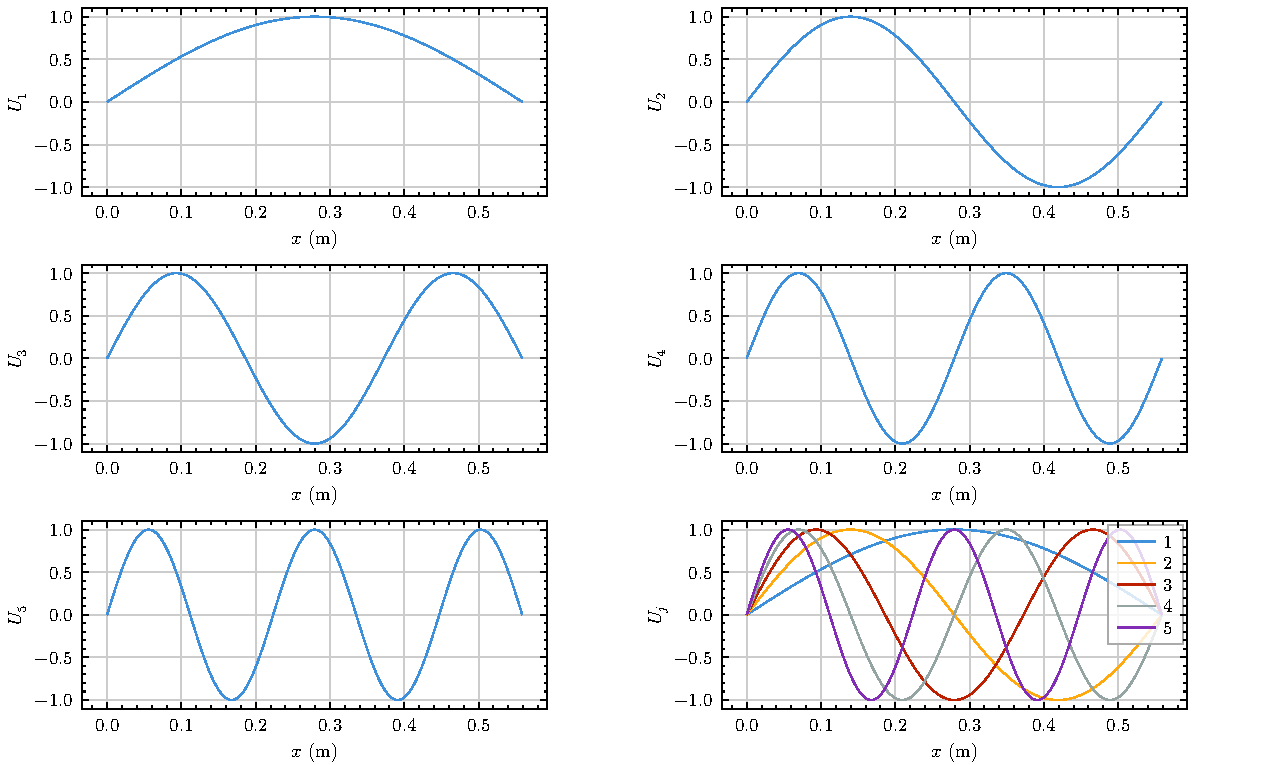
\includegraphics[width=0.95\linewidth]{figures/generated/solutions/A3.pdf}
\caption{Five string modes and their overlay.}\end{figure}
To check orthonormality in SI coordinates, use \(\phi_j=\sqrt{2/L}\,U_j\). The normalization factor is $\sqrt{2/L}=1.892\ \mathrm{m}^{-1/2}$. Each entry of the numerical check is the integral of a pair of scaled modes. Trapezoidal integration on the specified 1000 points gives the identity matrix to numerical precision,
\[
\int_0^L\phi_p\phi_q\,dx=\delta_{pq},\qquad
G\simeq\begin{bmatrix}1&0&0&0&0\\0&1&0&0&0\\0&0&1&0&0\\0&0&0&1&0\\0&0&0&0&1\end{bmatrix}.
\]
The unit-peak functions alone have diagonal integrals \(L/2\), whereas the scaled functions satisfy the orthonormality definition in the notes, PDF pages 154--158. The MATLAB script computes both the modes and the integrals.
\lstinputlisting[style=hwmatlab]{matlab/A3.m}
